
%(BEGIN_QUESTION)
% Copyright 2006, Tony R. Kuphaldt, released under the Creative Commons Attribution License (v 1.0)
% This means you may do almost anything with this work of mine, so long as you give me proper credit

Mange typer kjemisk analyse er basert på følsom deteksjon av lys. En av de mest følsomme enhetene for å konvertere et lyssignal til et elektrisk signal er en spesiell type elektronrør kalt et {\it photomultiplier tube}. Virkemåten bygger på den {\it fotoelektriske effekten}, der elektroner kan frigjøres fra en metalloverflate når et foton (en "partikkel" av lys) treffer overflaten:

$$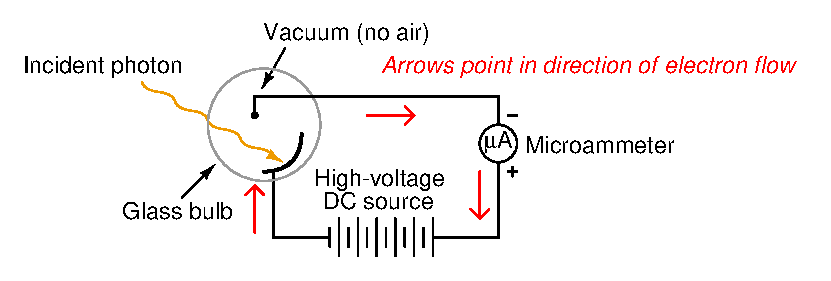
\includegraphics[width=15.5cm]{i00658x01.eps}$$

Et ekte photomultiplier-rør har imidlertid mer enn to elektroder. Det finnes katoden (den mest negative elektroden i røret), som emitterer elektroner når den treffes av innfallende fotoner. Anoden er den mest positive elektroden og samler elektroner i vakuumet. Mellom katoden og anoden finnes flere andre elektroder kalt {\it dynoder}, hver på et gradvis mer positivt potensial enn den forrige:

$$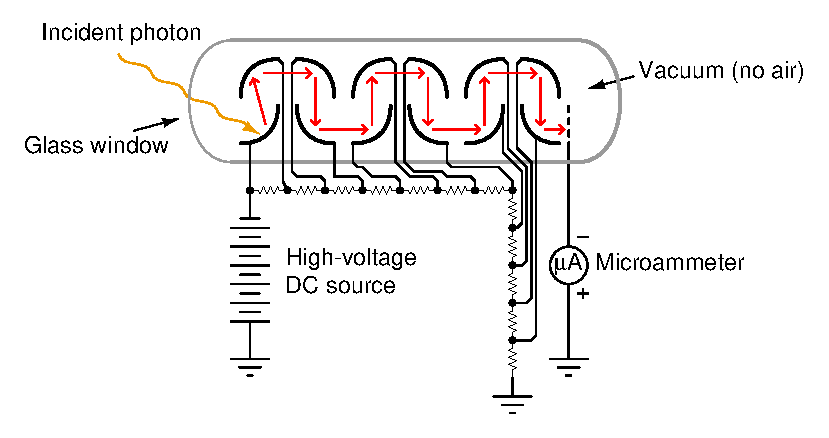
\includegraphics[width=15.5cm]{i00658x02.eps}$$

Identifiser elektrodene i illustrasjonen over, og beskriv deretter hensikten med alle disse dynodene.

\vskip 20pt \vbox{\hrule \hbox{\strut \vrule{} {\bf Forslag til sokratisk diskusjon} \vrule} \hrule}

\begin{itemize}
\item{} Hva tror du vil skje med {\it gain} i et photomultiplier-rør hvis DC-forsyningsspenningen synker? Forklar begrunnelsen din.
\item{} Hva tror du vil skje med ytelsen til photomultiplier-røret hvis en av spenningsdeler-motstandene får brudd? Forklar begrunnelsen din.
\end{itemize}

\underbar{file i00658no}
%(END_QUESTION)





%(BEGIN_ANSWER)

Dynodene har en effekt kalt {\it sekundæremisjon}, som "multipliserer" antallet elektroner som emitteres fra katoden. Jo flere dynoder, desto mer multiplikasjon, som kan komme opp i rundt 10$^{8}$.

%(END_ANSWER)





%(BEGIN_NOTES)

$$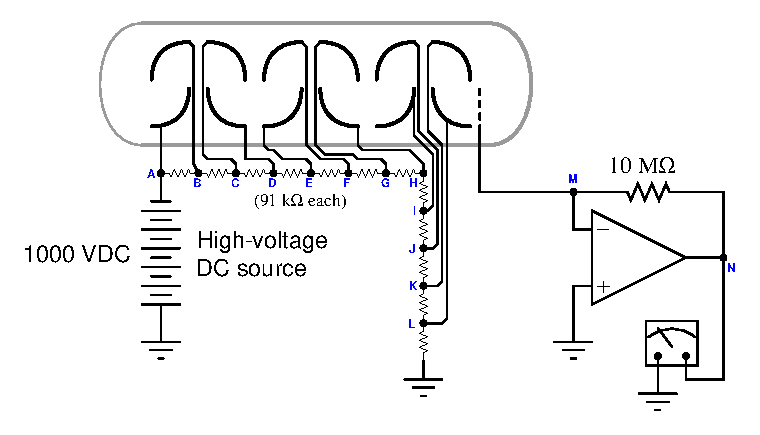
\includegraphics[width=15.5cm]{i00658x03.eps}$$

\vskip 20pt \vbox{\hrule \hbox{\strut \vrule{} {\bf Virtuell feilsøking} \vrule} \hrule}

Dette spørsmålet egner seg godt for en "Virtuell feilsøking"-øvelse. Presenter diagrammet for studentene, og tenk deg først en bestemt feil i systemet. Deretter presenterer du ett eller flere symptomer på feilen (noe en operatør eller bruker kan observere). Studentene foreslår så diagnostiske tester for å identifisere type og plassering av feilen, som om de var teknikere som feilsøker problemet. Din oppgave er å fortelle hva resultatet ville vært for hver foreslåtte test, og dokumentere resultatene slik at alle studentene ser dem.

Under og etter øvelsen er det nyttig å stille oppfølgingsspørsmål som:

\begin{itemize}
\item{} Hva forteller resultatet av siste diagnostiske test deg om feilen?
\item{} Anta at resultatet av siste diagnostiske test var annerledes. Hva ville det da fortalt deg om feilen?
\item{} Er siste diagnostiske test den beste vi kunne gjort?
\item{} Hva ville vært ideell testrekkefølge for å diagnostisere problemet med færrest mulig trinn?
\end{itemize}

%INDEX% Elektronikkrepetisjon: photomultiplier-rør

%(END_NOTES)
